% !TeX TXS-program:compile = txs:///pdflatex
\documentclass[10pt,xcolor={dvipsnames},french]{beamer}
\usepackage{xcolor}
\usepackage{cp-beamer}
\graphicspath{{./graphics/}}
\usetheme{Warsaw}
\hypersetup{pdfauthor={Pierquet},pdftitle={\currfilebase},pdfborder=0 0 0,allbordercolors=white}

%données
\logo{
\includegraphics[height=16pt]{flash}}
\title{Questions Flash, série n°1}
\author{1\up{ère} 2M2 - Droites (v1)}
\institute{\large Jeudi 18 Novembre 2021}
\date[18/11/2021]{\logossj \\ {\tiny Designé par \textcopyright{}\href{https://www.deviantart.com/dairon11/gallery/35504086/dragon-ball-kp}{Dairon11}}}
%\setbeamerfont{title}{size=\fontsize{28}{34}\bfseries}
\setbeamerfont{title}{size=\Huge\bfseries}
\setbeamerfont{author}{size=\LARGE}

%commandes utiles
\newcommand\haut[2]{\raisebox{-0.47ex}{\includegraphics[height=16pt]{goku_ssj#2}}\hfill{}Q#1}
\tikzstyle{every picture}+=[remember picture]
%essai en xparse ;-)
\NewDocumentCommand\noeud{ s m m }{%
	\tikz[remember picture,baseline=(#2.base)] \node[line width=0pt,inner sep=0pt,outer sep=2pt] (#2) {\IfBooleanTF{#1}{\ensuremath{#3}}{#3}};%
	}
%\newcommand\noeud[2]{\tikz[remember picture,baseline=(#1.base)]\node[line width=0pt,inner sep=0pt,outer sep=2pt] (#1){#2};}
%\newcommand\noeudm[2]{\tikz[remember picture,baseline=(#1.base)]\node[line width=0pt,inner sep=0pt,outer sep=2pt] (#1){\ensuremath{#2}};}
% utilisation de \pause ou de \onside<...>

%numérotation des diapositives
\newcounter{diapo}

\begin{document}

%page de titre
\begin{frame}
	\titlepage
\end{frame}

%nouvelle diapo
\stepcounter{diapo}
\begin{frame}{\haut{\thediapo}{0}}
	\begin{block}{Question n°\thediapo}
		La fonction $f(x)={\color<2>[rgb]{1,0,0} \noeud*{q1a}{\dfrac{2}{3}}}x+{\color<2>[rgb]{0,0,1} \noeud{q1b}{1}}$ est une fonction affine ?
		
		\begin{itemize}
			\item VRAI ?
			\item FAUX
		\end{itemize}
	\end{block}
	\pause
	\begin{alertblock}{Réponse n°\thediapo}
		C'est VRAI, on reconnaît la forme $mx+p$ avec $m={\red \noeud*{q1c}{\dfrac{2}{3}}}$ et $p=\noeud{q1d}{\blue 1}$.
	\end{alertblock}
	\begin{tikzpicture}
		\path[overlay,->,>=Stealth,red,densely dashed,line width=0.75pt](q1c.north) edge[out=110,in=-110] (q1a.south);
		\path[overlay,->,>=Stealth,blue,densely dashed,line width=0.75pt](q1d.north) edge[out=80,in=-80] (q1b.south);
	\end{tikzpicture}
\end{frame}

%nouvelle diapo
\stepcounter{diapo}
\begin{frame}{\haut{\thediapo}{0}}
	\begin{block}{Question n°\thediapo}
		La droite $\mathcal{D}$ d'équation réduite $y=2x+12$ passe par le point de coordonnées $({\color<2>[rgb]{1,0,0}\noeud{q2a}{$-10$}}\,;\,{\color<2>[rgb]{0,0,1}\noeud{q2b}{$-7$}})$.
		
		\begin{itemize}
			\item VRAI ?
			\item FAUX
		\end{itemize}
	\end{block}
	\pause
	\begin{alertblock}{Réponse n°\thediapo}
		On remplace \noeud{q2c}{\red $x$} par \noeud{q2d}{\red $-10$} et on obtient
		
		\hfill$y=2 \times ({\red -10})+12 = -20+12=-8 \neq$ \noeud{q2e}{\blue$-7$}.\hfill~
		
		\smallskip
		
		Donc c'est FAUX.
	\end{alertblock}
	\begin{tikzpicture}
		\path[overlay,->,>=Stealth,red,densely dashed,line width=0.75pt](q2c.north) edge[out=80,in=-80] (q2a.south);
		\path[overlay,->,>=Stealth,blue,densely dashed,line width=0.75pt](q2e.north) edge[out=90,in=-90] (q2b.south);
	\end{tikzpicture}
\end{frame}

%nouvelle diapo
\stepcounter{diapo}
\begin{frame}{\haut{\thediapo}{0}}
	\begin{block}{Question n°\thediapo}
		La fonction $g$ définie par $g(x)={\color<2>[rgb]{1,0,0} \noeud{q3a}{2}}x-2$ est :
		
		\begin{itemize}
			\item croissante ?
			\item décroissante ?
			\item constante ?
		\end{itemize}
	\end{block}
	\pause
	\begin{alertblock}{Réponse n°\thediapo}
		La fonction $g$ est affine, avec $\noeud{q3b}{\red m=2}\,\oplus$, donc elle est \textbf{croissante}.
	\end{alertblock}
	\begin{tikzpicture}
		\path[overlay,->,>=Stealth,red,densely dashed,line width=0.75pt](q3b.north) edge[out=45,in=-135] (q3a.south);
	\end{tikzpicture}
\end{frame}

%nouvelle diapo
\stepcounter{diapo}
\begin{frame}{\haut{\thediapo}{1}}
	\begin{block}{Question n°\thediapo}
		Une équation de la droite $\mathcal{D}$ tracée ci-dessous est :
		
		\begin{itemize}
			\item $y=-0,5x+1$ ?
			\item $y=-2x+1$ ?
		\end{itemize}
	
		\begin{center}
			\tunits{0.75}{0.75}
			\tdefgrille{-3}{3}{1}{0.5}{-1}{2}{1}{0.5}
			\begin{tikzpicture}[x=\xunit cm,y=\yunit cm]
				\tgrilles ;
				\tgrillep ;
				\draw[line width=1pt,->] (\xmin,0) -- (\xmax,0) ;
				\draw[line width=1pt,->] (0,\ymin) -- (0,\ymax) ;
				\foreach \x in {-3,-2,...,2} \draw[line width=1pt] (\x,4pt) -- (\x,-4pt) ;
				\foreach \y in {-1,0,1} \draw[line width=1pt] (4pt,\y) -- (-4pt,\y) ;
				\draw (1,-4pt) node[below] {\small $1$} ;
				\draw (-4pt,1) node[left] {\small $1$} ;
				\clip (\xmin,\ymin) rectangle (\xmax,\ymax) ;
				\draw[line width=1pt,blue,domain=-3:3] plot (\x,{-0.5*\x+1}) ;
				\onslide<2>{%
					\draw[red,line width=1pt,densely dashed,->,>=Stealth] (0,1) -- (2,1) node[red,midway,above] {\small $DH=2$};
					\draw[red,line width=1pt,densely dashed,->,>=Stealth] (2,1) -- (2,0) node[red,midway,right] {\small $DV=-1$};
					\filldraw[ForestGreen] (0,1) circle(2pt) ;
					\node (q4a) at (2,1) {} ;
					\node (q4b) at (0,1) {} ;
				}
			\end{tikzpicture}
		\end{center}
	\end{block}
	\pause
	\begin{alertblock}{Réponse n°\thediapo}
		On lit \og directement \fg{} \noeud{q4c}{\textcolor{ForestGreen}{$p=1$}} et {\red $m=\dfrac{DV}{DH}=\dfrac{-1}{2}=\noeud{q4d}{$-0,5$}$}.
		
		L'équation est donc $y=-0,5x+1$.
	\end{alertblock}
	\begin{tikzpicture}
		\path[overlay,->,>=Stealth,ForestGreen,densely dashed,line width=0.75pt](q4c.north) edge[out=80,in=-100] (q4b.south);
		\path[overlay,->,>=Stealth,red,densely dashed,line width=0.75pt](q4d.north east) edge[out=20,in=20] (q4a.north east);
	\end{tikzpicture}
\end{frame}

%nouvelle diapo
\stepcounter{diapo}
\begin{frame}{\haut{\thediapo}{1}}
	\begin{block}{Question n°\thediapo}
		Le tableau de signes de la fonction $h(x)=-2x-5$ est :
		\begin{center}
			\begin{tikzpicture}
				\tkzTabInit[]{$x$/0.75,$h(x)$/0.75}{$-\infty$,${-2,5}$,$+\infty$}
				\tkzTabLine{,{\only<1>{-}}{\only<2>{\red+}},z,{\only<1>{+}}{\only<2>{\red-}},}
			\end{tikzpicture}
		\end{center}
		\begin{itemize}
			\item VRAI ?
			\item FAUX ?
		\end{itemize}
	\end{block}
	\pause
	\begin{alertblock}{Réponse n°\thediapo}
		La fonction $h$ est une fonction affine :
		\begin{itemize}
			\item $h(x)=0 \ssi -2x-5=0 \ssi x=-2,5$
			\item $m=-2\,\ominus$, donc le signe après le \og zéro \fg{} est {\red \noeud{q5b}{$\ominus$}}.
		\end{itemize}
		\begin{tikzpicture}
			\path[overlay,->,>=Stealth,red,densely dashed,line width=0.75pt](q5b.north) edge[out=75,in=-105] ($(M22)!0.33!(M21)$.south);
		\end{tikzpicture}
		C'est donc FAUX.
	\end{alertblock}
\end{frame}

%nouvelle diapo
\stepcounter{diapo}
\begin{frame}{\haut{\thediapo}{1}}
	\begin{block}{Question n°\thediapo}
		Une équation de la droite $\mathcal{D}$  tracée ci-dessous est :
		
		\begin{itemize}
			\item $y=1,5$ ?
			\item $x=1,5$ ?
		\end{itemize}
		\begin{center}
			\tunits{0.75}{0.75}
			\tdefgrille{-2}{2}{1}{0.5}{-2}{2}{1}{0.5}
			\begin{tikzpicture}[x=\xunit cm,y=\yunit cm]
				\tgrilles ;
				\tgrillep ;
				\draw[line width=1pt,->] (\xmin,0) -- (\xmax,0) ;
				\draw[line width=1pt,->] (0,\ymin) -- (0,\ymax) ;
				\foreach \x in {-2,-1,0,1} \draw[line width=1pt] (\x,4pt) -- (\x,-4pt) ;
				\foreach \y in {-2,-1,0,1} \draw[line width=1pt] (4pt,\y) -- (-4pt,\y) ;
				\draw (1,-4pt) node[below] {\small $1$} ;
				\draw (-4pt,1) node[left] {\small $1$} ;
				\draw[line width=1pt,blue] (1.5,-2) -- (1.5,2) ;
				\onslide<2>{%
					\node (q6b) at (1.5,0) {} ;
				}
			\end{tikzpicture}
		\end{center}
	\end{block}
	\pause
	\begin{alertblock}{Réponse n°\thediapo}
		La droite $\mathcal{D}$ est une droite {\blue verticale}, son équation est donc \noeud{q6a}{\red $x=1,5$}.
		\begin{tikzpicture}
			\path[overlay,->,>=Stealth,red,densely dashed,line width=0.75pt](q6a.north) edge[out=75,in=-30] (q6b.south east);
		\end{tikzpicture}
	\end{alertblock}
\end{frame}

\end{document}